\chapter{Création et contrôle de la table Hive RAW}

\section{Schéma retenu}

Le CSV ne contient aucune virgule ni guillemet à l'intérieur d'un
champ (vérifié : chaque ligne compte exactement 24 virgules pour 25
colonnes), donc un \texttt{SerDe} délimité simple suffit, sans recourir
à \texttt{OpenCSVSerde}. Colonnes typées directement en DDL
(\texttt{INT}/\texttt{DOUBLE}/\texttt{STRING}) plutôt que tout en
\texttt{STRING}, pour bénéficier du cast automatique de Hive et
détecter d'éventuelles valeurs non numériques via des \texttt{NULL}.

\section{CREATE EXTERNAL TABLE}

Le script SQL de création est versionné. Il déclare les 25 colonnes
avec leurs types (\texttt{INT}, \texttt{DOUBLE}, \texttt{STRING}),
utilise un \texttt{SerDe} délimité simple avec le séparateur virgule,
pointe vers la zone \texttt{raw} de HDFS et ignore la ligne d'en-tête
via la propriété \texttt{skip.header.line.count} positionnée à
\texttt{1}.

\section{Contrôle de la table}

Exécuté via Beeline sur HiveServer2 :

\begin{verbatim}
SELECT COUNT(*) AS n, ROUND(AVG(annual_salary_usd),2) AS avg_sal
FROM projet_ia.ai_jobs_raw;

+-------+-----------+
|   n   |  avg_sal  |
+-------+-----------+
| 1500  | 194892.0  |
+-------+-----------+
\end{verbatim}

Le \texttt{COUNT(*)} vaut bien \textbf{1500} via Hive/Beeline. La
propriété \texttt{skip.header.line.count} fonctionne correctement pour
le moteur d'exécution Hive natif (Hive-on-MR).

\begin{figure}[h]
\centering
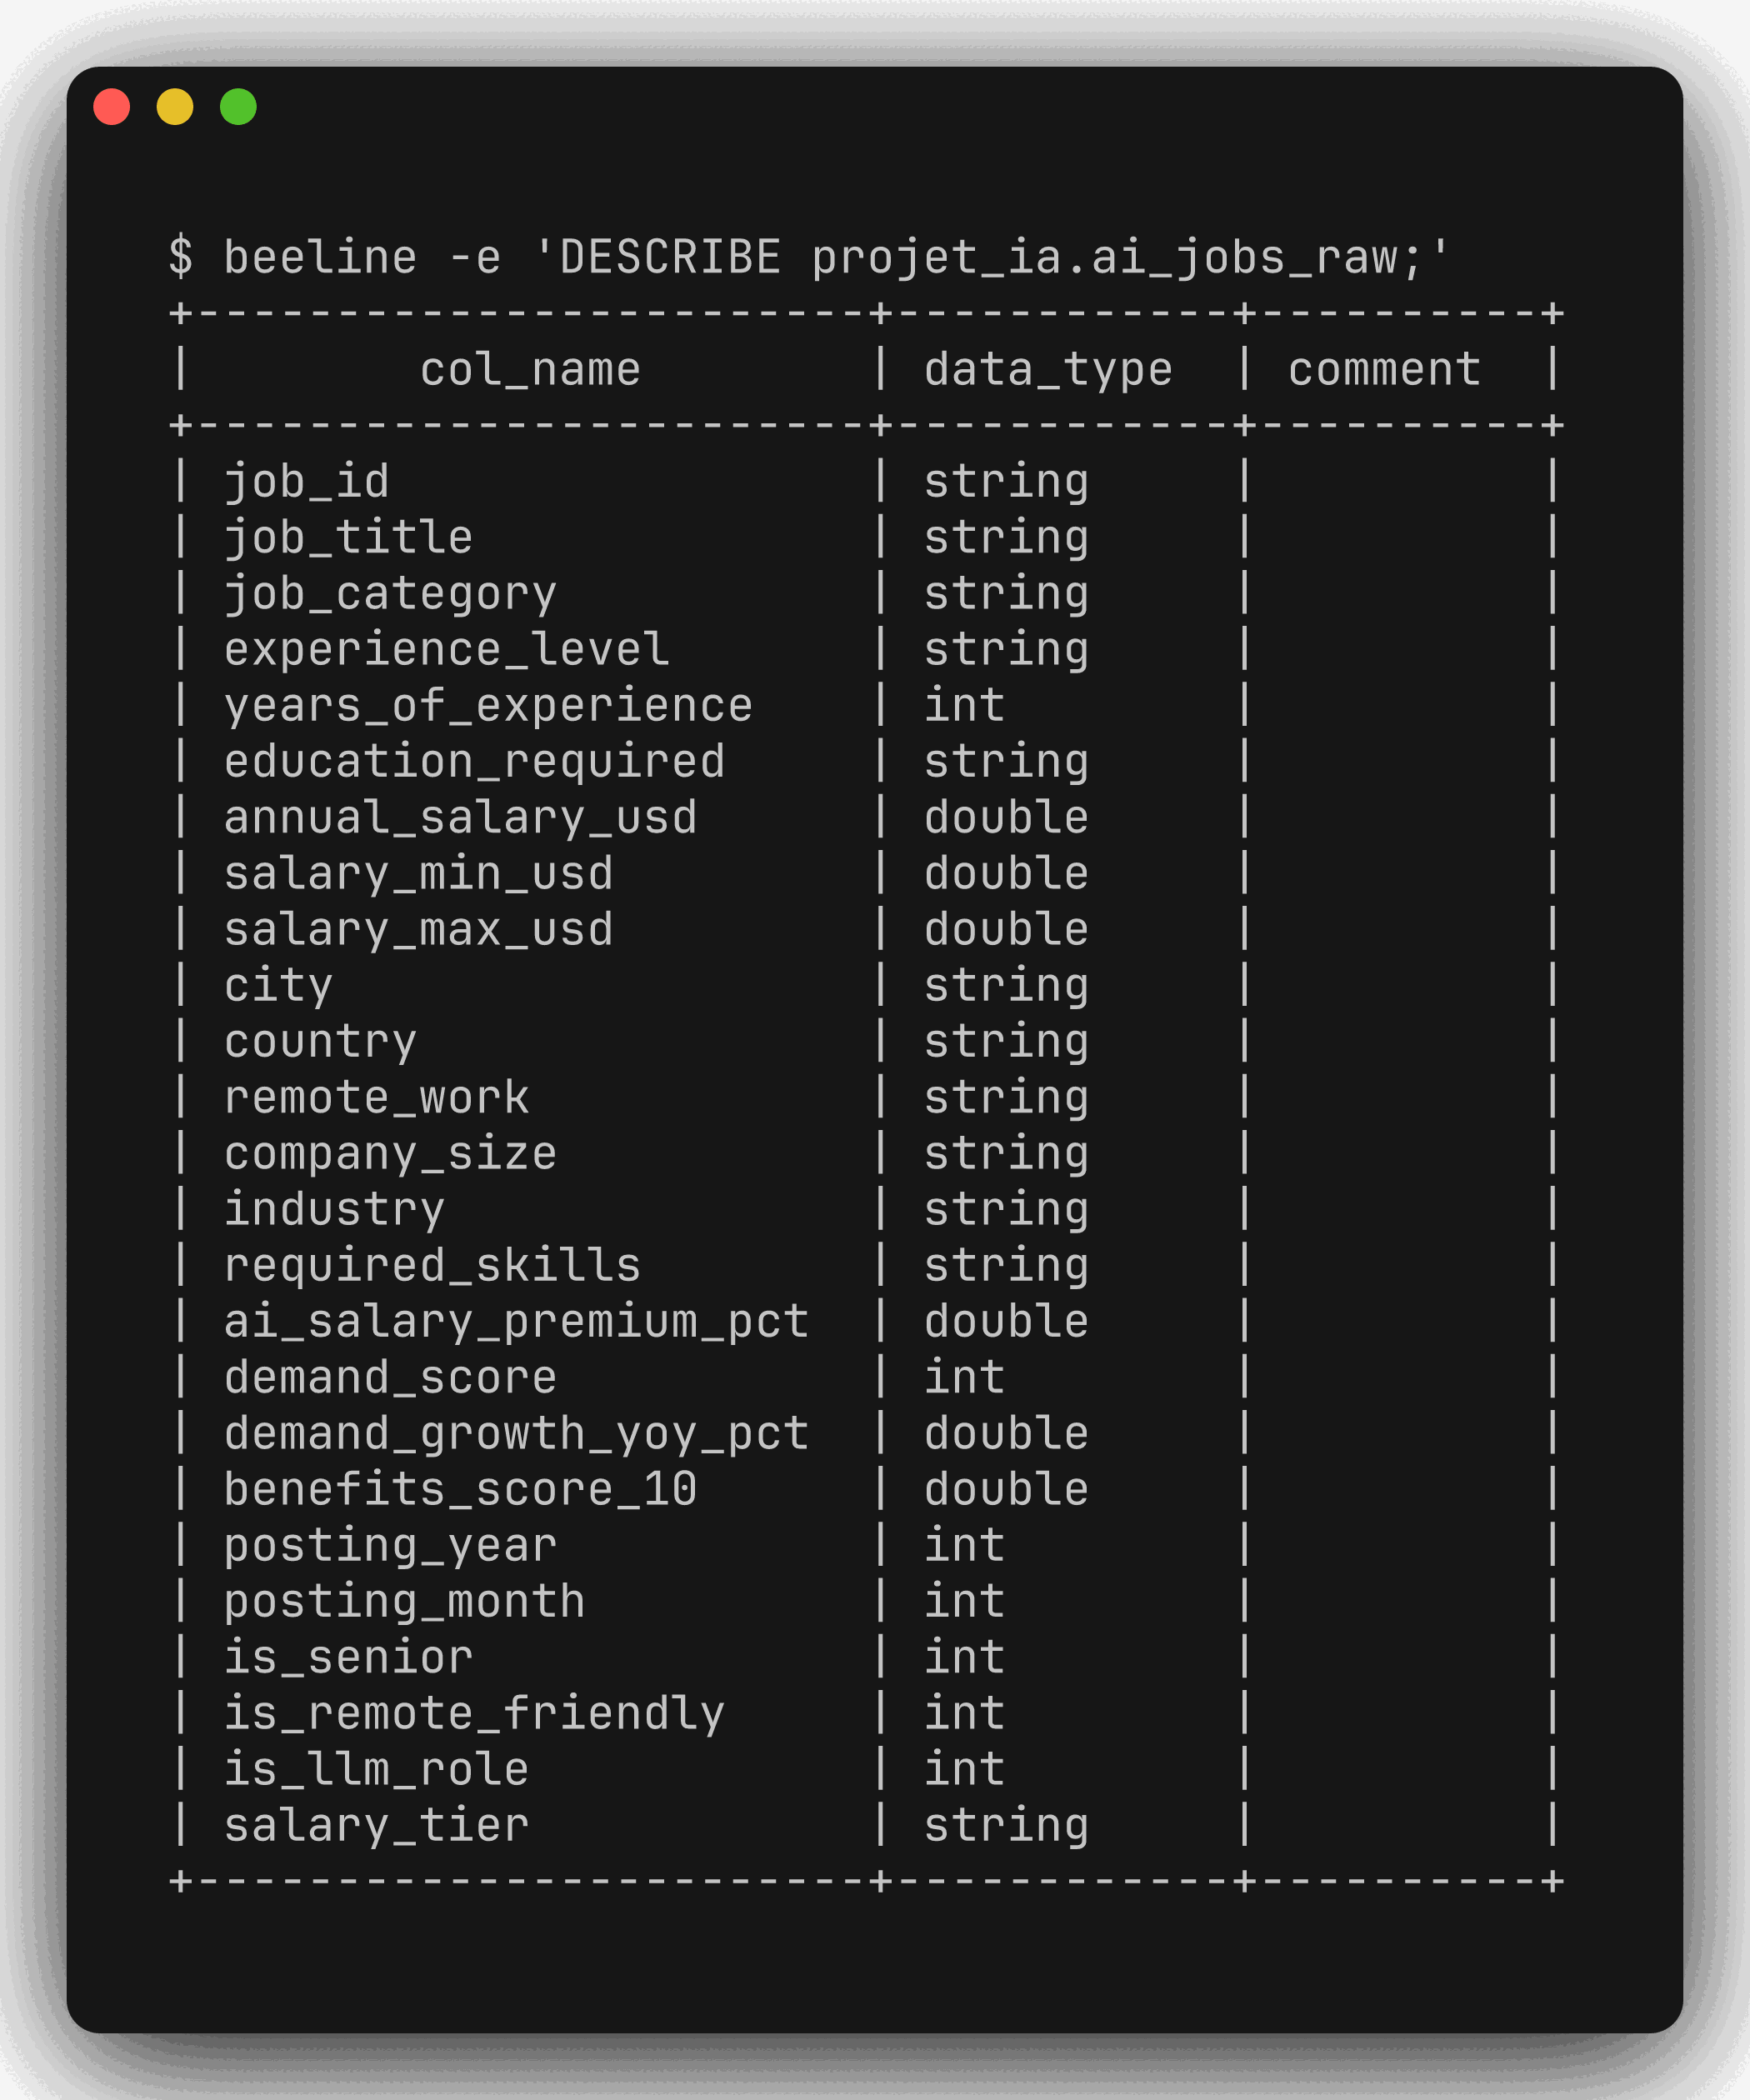
\includegraphics[width=0.85\linewidth]{figures/etape2_hive_raw_describe.png}
\caption{Schéma de la table Hive RAW (25 colonnes typées).}
\end{figure}

\begin{figure}[h]
\centering
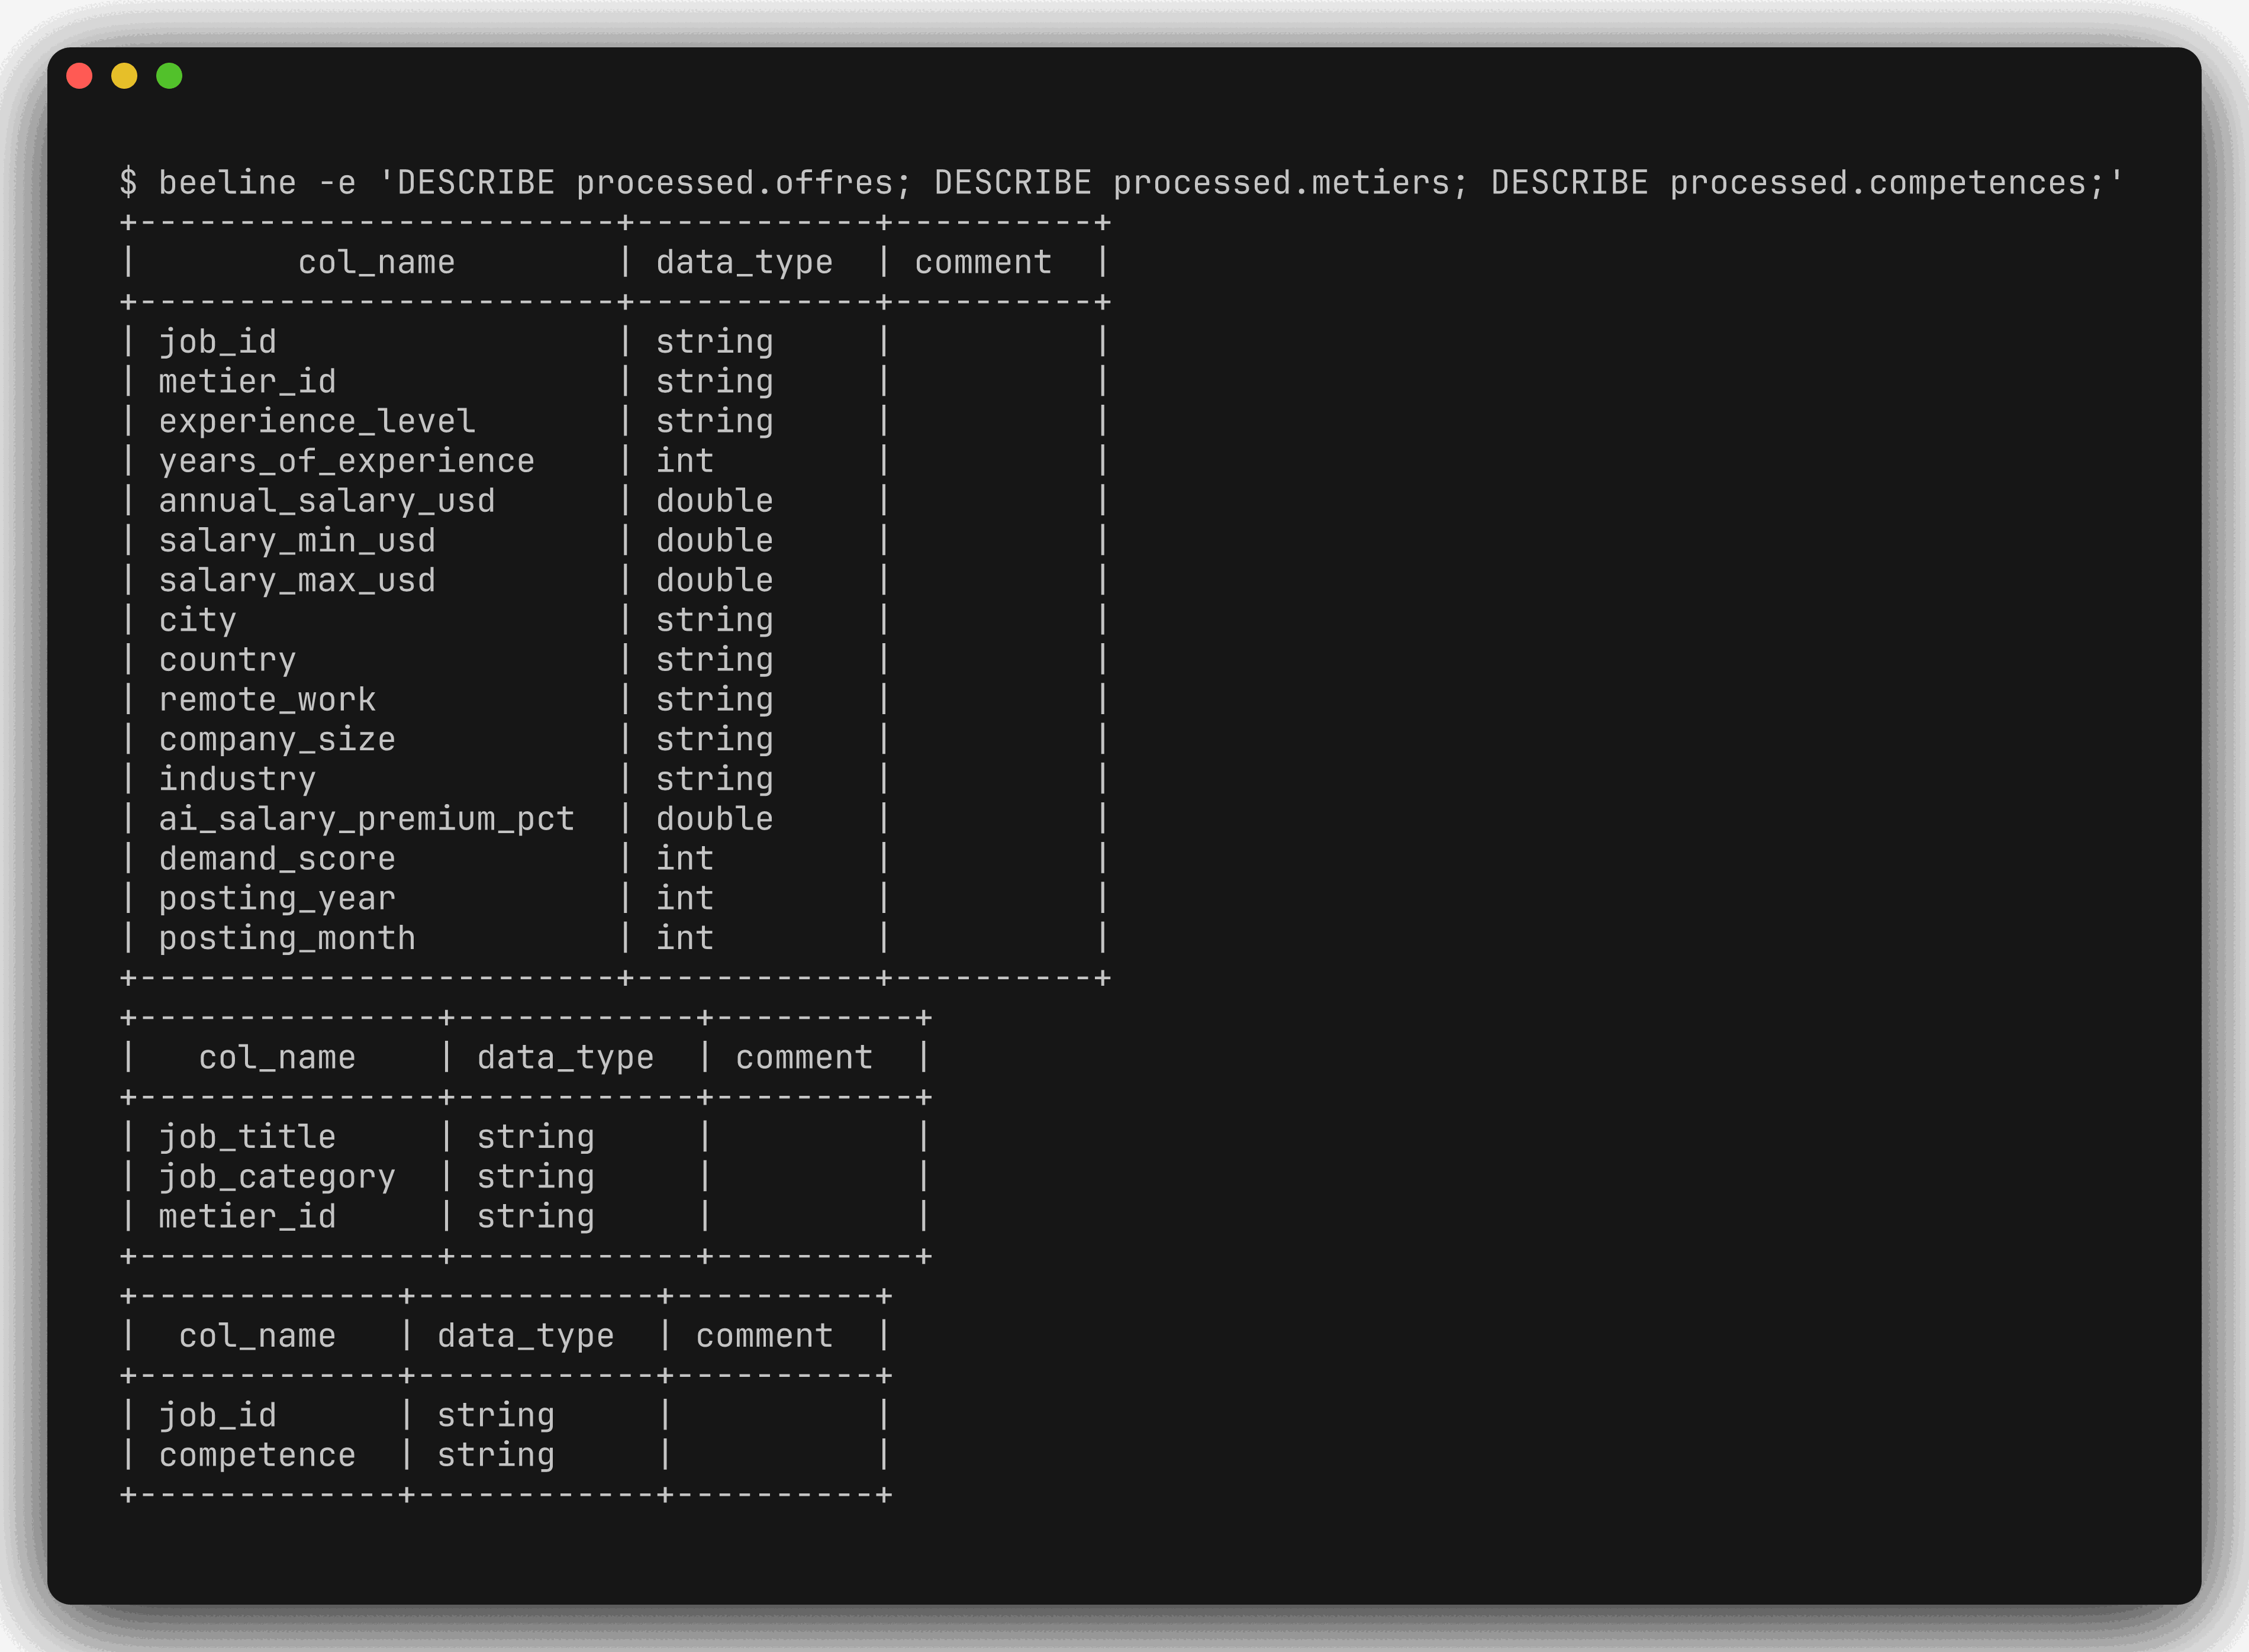
\includegraphics[width=0.85\linewidth]{figures/etape2_processed_tables_describe.png}
\caption{Schéma des tables \texttt{processed} (offres, metiers,
competences).}
\end{figure}

\begin{figure}[h]
\centering
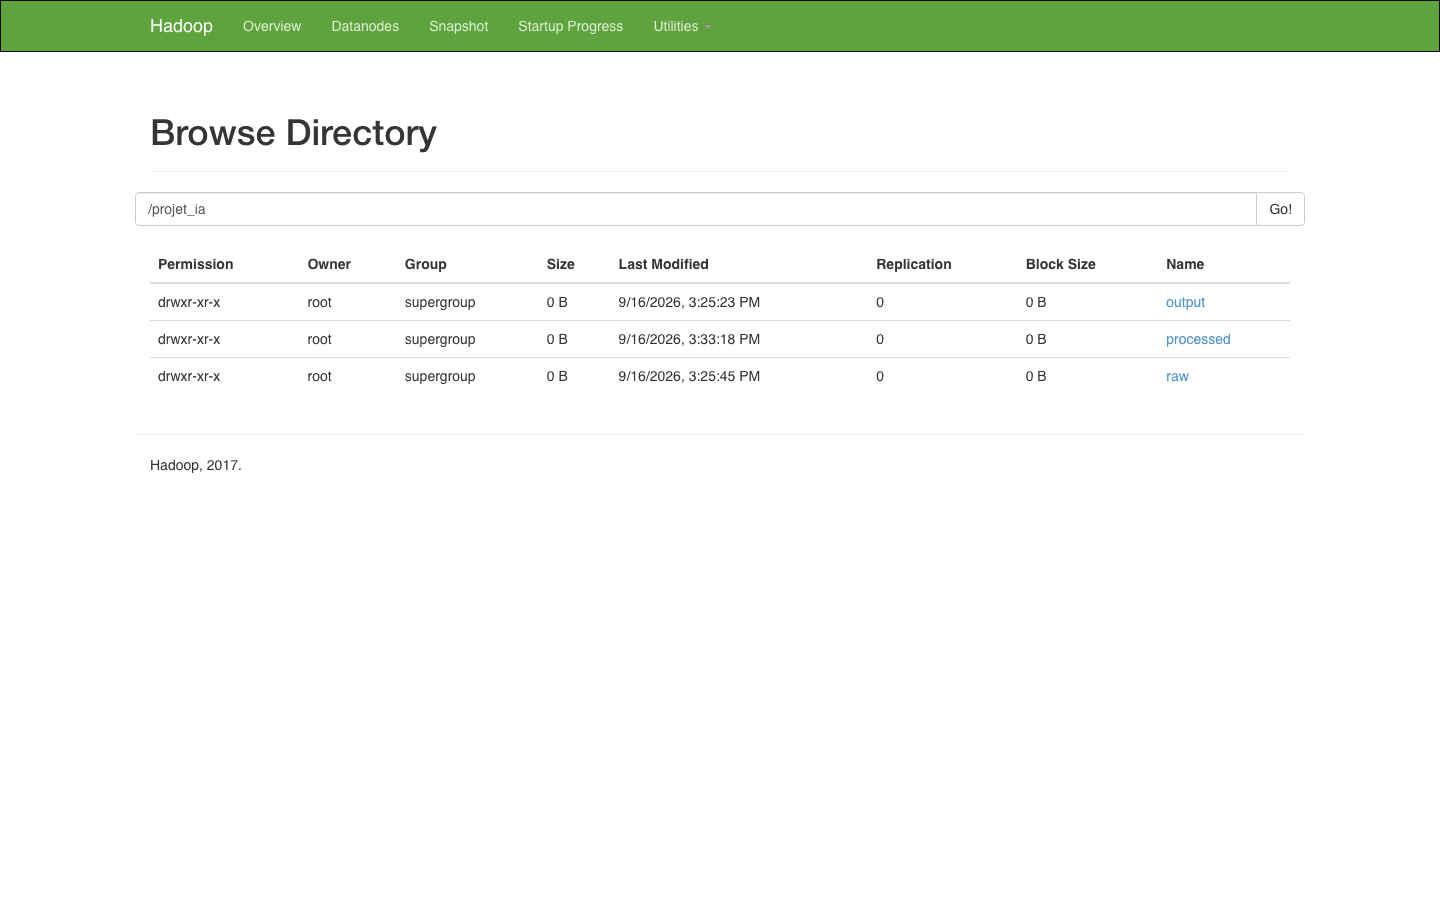
\includegraphics[width=0.85\linewidth]{figures/etape2_hdfs_namenode_explorer.png}
\caption{Interface web HDFS NameNode, arborescence
\texttt{/projet\_ia} (\texttt{raw}, \texttt{processed}, \texttt{output}).}
\end{figure}
